% Created 2023-11-05 Sun 19:41
% Intended LaTeX compiler: pdflatex
\documentclass[11pt]{article}
\usepackage[utf8]{inputenc}
\usepackage[T1]{fontenc}
\usepackage{graphicx}
\usepackage{longtable}
\usepackage{wrapfig}
\usepackage{rotating}
\usepackage[normalem]{ulem}
\usepackage{amsmath}
\usepackage{amssymb}
\usepackage{capt-of}
\usepackage{hyperref}
\usepackage[margin=1in]{geometry}
\usepackage{customTitle}
\project{}
\supervisor{Dr. Sandeep \textsc{Neema}}
\let\oldsection\section
\renewcommand\section{\clearpage\oldsection}
\usepackage[parfill]{parskip}
\setcounter{secnumdepth}{0}
\author{Benjamin Van Sleen}
\date{November 6, 2023}
\title{LLModelica\\\medskip
\large Investigating LLM capacity for composition in systems design}
\hypersetup{
 pdfauthor={Benjamin Van Sleen},
 pdftitle={LLModelica},
 pdfkeywords={},
 pdfsubject={},
 pdfcreator={Emacs 30.0.50 (Org mode 9.6.9)}, 
 pdflang={English}}
\begin{document}

\maketitle
\tableofcontents




\section{Introduction}
\label{sec:org96a5dc2}
\begin{abstract}
Over the past year, LLMs have demonstrated signficant usefulness by generating code. There have been many applications exhibiting LLM-generated web components and simple software applications. However, the extent to which they can be used for composition in systems design is still unclear; to date, most LLM-based applications are focused on serving as a ``programmer's assistant'' -- this project instead aims to explore the feasibility of using LLMs as an ``engineer's assistant''.

Similar work in the programming domain is typically centered around allowing an LLM to freely access and interact with a sandboxed container. In this container, the LLM has free-reign to generate and execute code, manipulate the filesystem, and interact with the network. Instead, this project aims to allow the LLM similar free-reign to a proxy for real-world, physical systems: Modelica's simulation engine. This project explores the extent to which LLMs can be used to generate and manipulate Modelica models in a way that is useful for compositional systems design.

The goal is: can an engineer simply dictate the desired behavior of a physical system and have the implementation details be automatically generated? In short, yes. GPT-4 shows significant promise in applying its ``understanding'' of physical systems through composing units of the Modelica Standard Library.
\end{abstract}

Large language models (LLMs) optimized for human-interaction (e.g. ``chat'' models) have taken the programming world by storm in recent months. ChatGPT and GitHub Copilot have demonstrated that LLMs can be used to generate useful code snippets and even entire programs. As these tools have moved from proof-of-concepts to real-world products, the question of their abilities to generalize to the usage of out-of-training-distribution (OOD) proprietary libraries, APIs, and codebases has become increasingly important.

These chat-based LLMs have an aptitude for explaining the behavior of complex physical (i.e. non-software) systems. While the pedagogical applications are self-evident, a new question arises: can these models' ``understanding'' of physical systems be leveraged to create a Copilot-like tool for systems design engineers?

Systems engineers frequently make use of software platforms such as Mathworks' Simulink or the open-sourced Modelica to design and simulate complex physical systems. These platforms expose a graphical interface for the user to compose a system from a library of components. The user can then simulate the system and analyze its behavior. This composition of smaller subcomponent blocks is critical to the design process, as it allows for the designer to create higher levels of abstraction built upon firm interface guarantees. For an LLM to be a useful and effective design engineer's assistant, it is essential for it to be able to compose systems from a library of components -- many of which are OOD.

This paper presents a tool for qualitatively investigating GPT-4's ability to implement Modelica components subject to an English description of the component's behavior and an associated Modelica unit test. Due to the author's academic background, the tool's performance has been mostly evaluated within the domain of electrical systems and circuitry, but the tool is generalizable to any domain that can be represented in Modelica.

\section{Tool Usage and Implementation}
\label{sec:org6f69565}
For the tool to be useful, it should be enough to simply describe the overall behavior of a system and have the implementation details automatically generated. The tool should choose reasonable default values for any unspecified parameters, and it should be relatively easy to iterate and improve upon the generated design from within the tool. LLModelica is designed to accept an input file containing a specification of a desired behavior and a unit test for that behavior. The tool then autonomously generates a Modelica component that satisfies the specification and passes the unit test; the generated component can be further modified or refined by interactive, high-level natural language feedback from the user. Any particular interface requirements can be specified in this input file, and the tool will ensure that the generated component satisfies those requirements.

\subsection{Usage}
\label{sec:org3eba5ba}
LLModelica is designed to allow GPT-4 as much freedom to explore and tinker with its design as safely possible. Taking advantage of the \texttt{OMPython} Python API for OpenModelica, LLModelica is a middleman facillitating the interaction between GPT-4 and the Modelica compiler. The initial user specification is parsed and passed to GPT-4, which generates a Modelica component. This component is then compiled; if the compilation fails, the error message is sent back to GPT-4 in the same ``chain'' of context, and GPT-4 will attempt to autonomously debug and fix the compilation error. If the compilation succeeds, the unit test is run; if the unit test fails, the error message is sent back to GPT-4 in the same manner as above. Finally, if all of these steps succeed and the generated component appears to pass the given unit test, the component definition and any results or plots from the unit test are returned to the user.

At this point, the user can choose to either accept the generated component or provide feedback to GPT-4 in the form of a natural language description of the desired changes. Importantly, this feedback can either be low-level and specific (e.g. change the resistance of R1 to 100 ohms) or higher-level and functional: roughly the same level of guidance one would give to an undergraduate in the field (e.g. ensure the output impedance of the component is effectively infinite to prevent loading effects). This feedback is then passed to GPT-4, which generates a new component definition. This component is then compiled and tested as before, and the results are returned to the user. This process will be repeated until the user is satisfied with the generated component.

\subsection{Implementation}
\label{sec:org804c71b}
\begin{center}
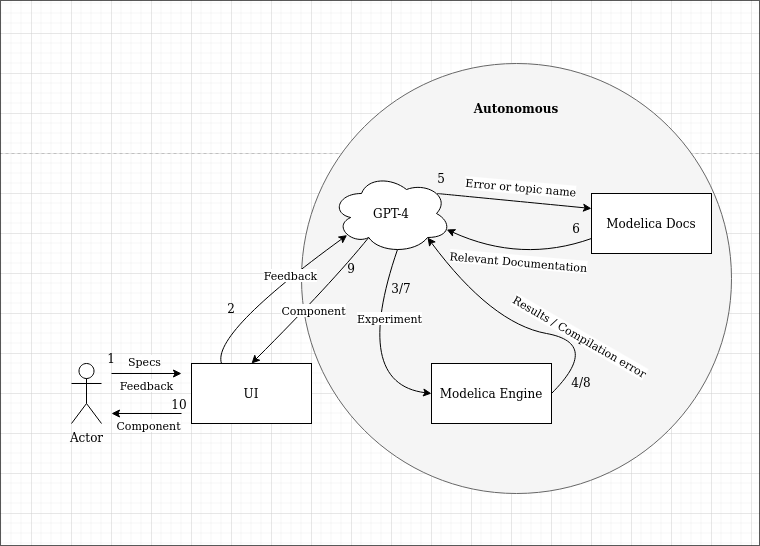
\includegraphics[width=3in]{./images/diagram.png}
\captionof{figure}{LLModelica architecture}
\end{center}

LLModelica relies heavily on the June 13, 2023, snapshot of the GPT-4 model; this particular model snapshot was trained to perform a function-calls. This ``function-calling'' allows for the API caller to pass a series of function descriptions and associated parameters (each with their own descriptions). The API will then respond with a JSON object containing the name of the function the LLM chooses to call and the parameters it chooses to pass to that function. LLModelica will, in turn, respond back to the API with the (string) output of that function call. This mechanism of allowing for GPT-4 to remotely execute commands is the backbone of LLModelica's implementation; consequently, the tool is highly dependent on the GPT-4 API. LLModelica exposes four main functions to the GPT-4 function-calling API: \texttt{define\_model}, \texttt{simulate}, \texttt{plot}, and \texttt{modelica\_documentation}.

The \texttt{define\_model} function is the primary function of the tool, and it is responsible for instantiating a generated Modelica component definition. \texttt{define\_model} accepts a \texttt{pydantic} object model representing the Modelica model specification. Over the course of LLModelica's development, the model specification was initially constrained as an attempt to reduce the search space for GPT-4. It was broken into specific fields: the name of the component, the parameters the component would utilize (e.g. ``Modelica.Units.SI.Velocity v = 10''), and the differential equations governing the parameters' relationships with one another (e.g. ``der(x) = v''). However, over time, it became clear that this approach was too restrictive; GPT-4 frequently misunderstood this separation and would confuse parameter declarations with equations. The model specification was then cut down to two fields: the name of the model, and a single string representing the entire component definition. To the author's surprise, allowing GPT-4 a greater degree of freedom in defining its own components drastically reduced the number of syntax and compilation errors. Should the component definition fail to compile or instantiate, LLModelica will return the error message to GPT-4. For simple syntactical errors, GPT-4 will frequently fix the error upon the next iteration. For more complex errors, GPT-4 will often ``give up'' and attempt to query the documentation associated with the library at hand.

LLModelica exposes a function to aid GPT-4 in its search for information outside its training distribution. The \texttt{modelica\_documentation} function accepts a string representing the model's desired search query. Frequently, GPT-4 will attempt to utilize a function or component that either no longer exists or has changed locations since the model's training. In these cases, GPT-4 will explicitly query the documentation for the missing component. Upon first launch, LLModelica will embed and store (utilizing a basic \texttt{Chroma} vectorstore) a specified Modelica library. Using the \texttt{langchain} Python package, the library is split along component definitions (or, if the component definition is too large, along the component's equations). The \texttt{modelica\_documentation} function will embed the search query, and return the \(k\) most cosine-similar components or equations (experimentally, a \(k\) of 1 or 2 typically outperforms larger sizes). This allows GPT-4 to ``search'' the documentation for the missing component, and, frequently, GPT-4 will be able to utilize the returned component in its design. It is important to note that LLModelica does not use the OpenAI embeddings API; instead, LLModelica performs all embedding and cosine similarity calculations locally using the \texttt{all-mpnet-base-v2} model from the \texttt{sentence-transformers} Python package. In the opinion of the author, the OpenAI embeddings API did not provide a significant enough improvement in performance to justify the additional API calls.

The \texttt{simulate} and \texttt{plot} functions allow for the execution and evaluation of the generated component's performance with respect to the given unit test. Some simulations result in numeric outputs; GPT-4 is perfectly capable of adjusting its model to ensure the component's output matches the expected output. However, some simulations are best represented with a plot. Since the rumored multi-modal GPT-4 API is not yet available, LLModelica allows the user to inspect the output plots and provide unstructured feedback. This feedback is then passed to GPT-4, which will attempt to adjust the component's equations to better match the desired plot. This process is repeated until the user is satisfied with the generated component.

\subsection{Prompt Structure}
\label{sec:org21961f0}
The OpenAI Chat models API is structured to accept three kinds of messages: user, assistant, and \emph{system}. The user and assistant messages are relatively straightforward; the user message is the message sent by the user, and the assistant message is the response generated by the LLM. The system message, however, governs the distribution of assistant message responses returned for a given set of input user messages. While the system message was present in the GPT-3.5 API endpoint, GPT-4 was trained to adhere significantly more closely to the system message. Slight differences in the system message can result in drastically different outputs from GPT-4. At least within the experimental setup of this project, a good system message contains several components: 1) grounding the LLM in the background knowledge that it should have (also known as ``expert'' prompting, or convincing it that it is an expert in the field); 2) providing a detailed description of the target audience; 3) providing detailed, positive descriptions of the desired types of outputs (``respond only in code and without ANY commentary''); and 4) providing detailed, negative descriptions of the unacceptable types of outputs (e.g. ``DO NOT assume the existence of any other external libraries or packages'').

After using the system message to generally improve the quality of the generated components, LLModelica uses the previously described \texttt{modelica\_documentation} lookup function to dynamically incorporate relevant information from the Modelica documentation into the user's initial prompt. The combination of the natural language behavioral description and the unit test is abbreviated for length and embedded as the query vector for the documentation lookup. Relevant documentation or actual model definitions are then inserted above the user's desired behavior when sent to the GPT-4 API.

Final prompt structure:

\begin{enumerate}
\item System message
\begin{enumerate}
\item ``Expert'' prompting setting expectations for quality of response
\item Description of target audience
\item Specific positive qualities of the types of desired outputs
\item Specific negative qualities of the types of undesired outputs
\end{enumerate}
\item Relevant documentation \& examples
\begin{enumerate}
\item The example component definitions or documentation excerpts most cosine-similar to the user's desired behavior are inserted
\end{enumerate}
\item User's desired behavior
\begin{enumerate}
\item The user's specific desired behavior; typically framed as one would instruct a talented high school or undergraduate student
\item Specificity is positively correlated with the quality of the generated component
\end{enumerate}
\item Mandatory interface guarantees the generated component must satisfy
\begin{enumerate}
\item For the component to be useful, it must coherently fit into the designer's broader vision
\item This is essential for the LLM to generate usefully composable subcomponents
\end{enumerate}
\item Unit test
\begin{enumerate}
\item Compilable model definition utilizing desired subcomponent in a way that maximally explores its functionality and adherence to the specification
\item LLModelica will stop autonomously iterating \& debugging definitions when the unit test is executed
\end{enumerate}
\end{enumerate}


\section{Qualitative Evaluation}
\label{sec:org1d54762}
The appropriate way to evaluate this particular tool is to compile a large-scale, Leetcode-style dataset of Modelica component - unit test pairs. Such evaluation suites are beginning to be created for the realm of LLM-generated software; unfortunately, no such dataset exists for Modelica or systems engineering components. Consequently, this paper will detail a qualitative evaluation of LLModelica's performance on a pair of simple circuits: passive and active low-pass filters.

\subsection{Passive Low-Pass Filter}
\label{sec:org7782fac}
To demonstrate the baseline competency of LLModelica in generating simple components following both functional and interface specifications, the tool was tasked with generating a passive low-pass filter. The user's desired behavior was as follows:

\begin{quote}
\textbf{Functional specification}: The \texttt{LowPass} component should filter out all input voltages with a frequency higher than the given breakpoint frequency. It should allow all input voltages with a frequency lower than the given breakpoint frequency to pass through unimpeded. The filtered signal should be available at the output pin (named "Vout").

\textbf{Interface}: \texttt{LowPass} should accept a voltage signal input at \texttt{LowPass.p}, and ground at \texttt{LowPass.n}, and the output (filtered) signal should be found at \texttt{LowPass.Vout.v}.
\end{quote}

The top-level, user-defined system is shown in Figure 1. Specifically, it attaches two sinusoidal voltage sources to the \texttt{LowPass} component in series. One voltage source has a ``high'' frequency, and the other has a ``low'' frequency. According to the user's desired behavior, the \texttt{LowPass} component should accept an input parameter governing the breakpoint frequency. In this circuit, the high-frequency input is set to 10 Hz, and the low-frequency input is set to 0.1 Hz. Both input signals have amplitudes of 12 V. The breakpoint frequency is set to 1 Hz.

\begin{center}
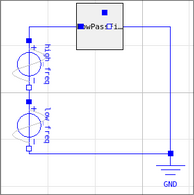
\includegraphics[width=3in]{./images/passive_lowpass_final_circuit.png}
\captionof{figure}{Final circuit ``composing'' passive low-pass filter}
\end{center}

\begin{center}
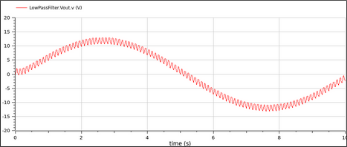
\includegraphics[width=3in]{./images/passive_lowpass_desired_output.png}
\captionof{figure}{Desired final output for passive low-pass filter}
\end{center}

If the \texttt{LowPass} component is functioning correctly, the output signal should be as close as possible to a sinusoid with an amplitude of 12 V and a frequency of 0.1 Hz (as shown in FIgure 2).

To avoid priming the LLM with the desired output, the above system was not included in the user's unit test; instead, a slightly different system was used as described in Figure 3. The unit test consists of two disconnected circuits: one with a high-frequency source and one with a low-frequency source. Ideally, the amplitude of the output of the \texttt{LowPass} component should be 0 V for the high-frequency source and 12 V for the low-frequency source.

\begin{center}
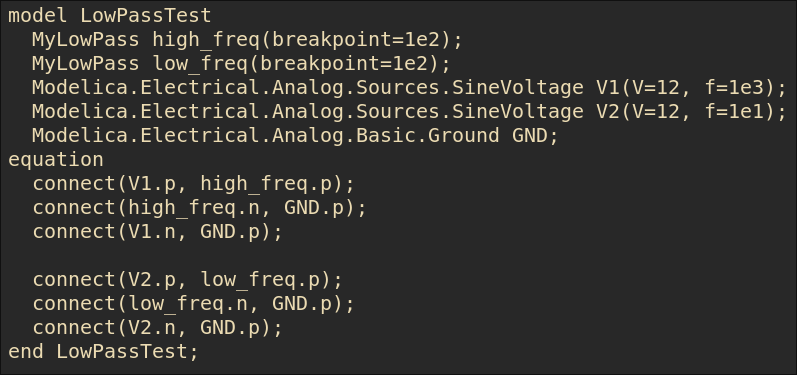
\includegraphics[width=3in]{./images/passive_lowpass_unit_test.png}
\captionof{figure}{Specification for unit test of passive low-pass filter passed to LLModelica}
\end{center}

\begin{center}
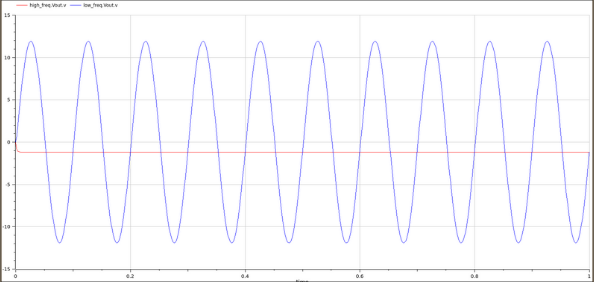
\includegraphics[width=3in]{./images/passive_lowpass_unit_test_output.png}
\captionof{figure}{Plotted output from LLModelica unit test}
\end{center}

After several iterations correcting compilation errors, the output of a successful generated model is depicted in Figure 4. Notably, in early attempts, the LLM attempted to use the nonexistent \texttt{Modelica.Electrical.Analog.Interfaces.VoltageSensor} component instead of\\[0pt]
\texttt{Modelica.Electrical.Analog.Sensors.VoltageSensor}, and it smartly used the \texttt{modelica\_documentation} lookup function to find the component's new module name. In the end, though, LLModelica correctly generated a low-pass filter that passed the unit test.

Due to Modelica's implementation, the generated component cannot yet be visualized in the GUI ``Connections Editor''; to render the component, the component definition must include ``annotations'' (e.g. ``annotation(Placement(transformation(extent=\{\{-10,10\},\{10,10\}\}, rotation=0)))'') that specify the component's visual appearance. Since the LLM has not yet been asked to generate these annotations, the component cannot be visualized in the GUI. Amazingly, though, at this point the user can simply ask (direct quote: ``add annotations to draw the connections''), and the LLM will generate the appropriate annotations and insert them into the existing component definition. The result can be seen in Figure 5.

\begin{center}
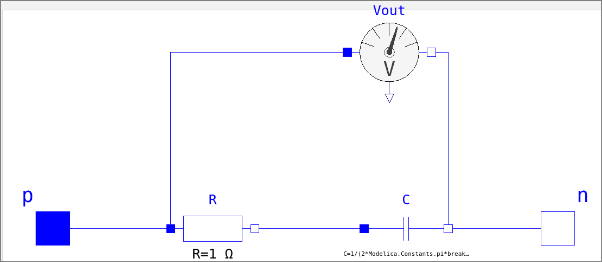
\includegraphics[width=3in]{./images/passive_lowpass_generated_v1.png}
\captionof{figure}{First LLModelica generated component passing unit test}
\end{center}

Now, interestingly enough, while the generated component does, in fact, pass the given unit test (with the filtered voltage at \texttt{LowPass.Vout.v}), it does not totally satisfy the user's initial specification -- at least in the way it was intended. The user asked for the output signal to be found on an output pin -- assuming it would be on a \texttt{Modelica.Electrical.Analog.Interfaces.PositivePin}. Instead, the LLM generated a component with the output signal found on a voltage sensor. In this particular context, this actually makes more sense: the voltage sensor is intended to be a read-only interface, and due to the low output impedance of the filter, it is not intended to be connected to any other components. In this case, the LLM has actually improved upon the user's specification, and the user can simply accept the generated component as-is. However, if the user is still not satisfied, they can simply ask ``Replace the voltage sensor with an output pin,''  and the LLM will generate a new component definition (and GUI annotations) that satisfies the user's specification. The result can be seen in Figure 6.

\begin{center}
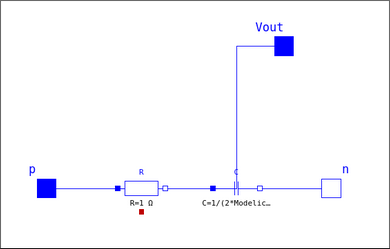
\includegraphics[width=3in]{./images/passive_lowpass_generated_v2.png}
\captionof{figure}{Final LLModelica generated component}
\end{center}

\begin{center}
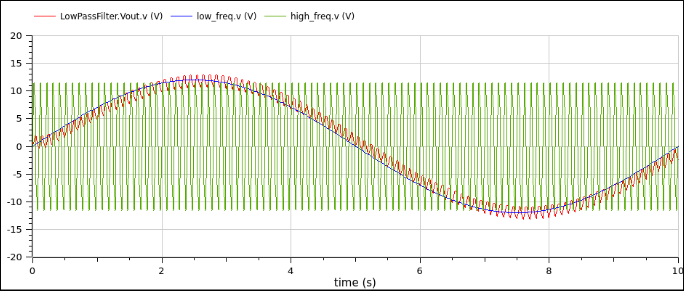
\includegraphics[width=3in]{./images/passive_lowpass_final_output.png}
\captionof{figure}{Simulated output of completed circuit with LLModelica generated component}
\end{center}

Finally, Figure 7 demonstrates that the generated component can be used in a larger system to achieve both the desired functionality and interface. As a bonus, the LLM even correctly generated the GUI annotation guides so the user can more closely inspect the generated component. The user can now use the generated component in any other system.

\section{Future work}
\label{sec:org775bc7a}
This application is still in its infancy; there is much left to be explored. In particular, this project did not extensively explore the many OpenAI API parameters. One parameter is particularly of note: this project primarily used low \texttt{temperature} settings (0.0 to 0.4) for the sake of simplicity, but higher temperatures (0.6 to 1.0) may be able to generate more creative solutions to more complex problems.

Future work should be directed at using this tool to solve increasingly difficult and complex problems. This paper heavily detailed the process of generating simple passive low-pass filters; the next step would be to compare performance on slighty more complex components (e.g. bandpass filters). Active low- and high-pass filters were successfully generated, but they required an unsatisfactory number of design iterations based upon human feedback. The author believes the limiting factor here was poor documentation lookup performance.

Further work can directly build upon this project by restricting GPT-4 to utilizing only a proprietary library of Modelica components. These would necessarily be out of the GPT pretraining sample, and thus the LLM would be forced to rely more heavily upon the RAG-based documentation lookups.

At the time of implementation, retrieval-augmented generation (RAG) systems were only beginning to be heavily explored. The methods used for documentation lookups and dynamic prompt augmentation are relatively simple; there is ample room to optimize and improve document retrieval to minimize noise and confusion for the LLM. This RAG could be additionally augmented by allowing access to non-Modelica domain-specific reference texts (e.g. an electrical engineering textbook) to allow for GPT-4 to research physical phenomena beyond its pretraining data.

Similarly, At the time of implementation, GPT-4 Vision was merely a rumor. While it is still not available via API, vision-augmented LLM generation could be used for myriad applications within LLModelica. Notably, one major shortcoming of the current implementation is that many unit-tests require visual inspection of plots or waveforms. With GPT-4 Vision, the LLM could critique its own generated components and automatically determine acceptability. This would allow for a much more streamlined development process with reduced continuous user feedback.
\end{document}